In this chapter, product architecture is described using 4 + 1 architectural view model \cite{Kruchten:1995:VMA:624610.625529}. It is based on the multiple concurrent views and therefore better explanation of architecture can be provided.
Only high level design will be presented in this chapter and in each sprint, specific, detailed architecture will be described.
The design is made with emphasis on generality, therefore it is possible, that in particular sprints in the architecture section it will be adapted to specific situation.

Since some design patterns were used, the purpose of using specific pattern and its advantages will be discussed in the end of this chapter.

\section{Logical view}
The description of the functional requirements of the architecture. The client and the server are decomposed into a set of key abstractions, taken(mostly) from the problem domain, in the form of objects or object classes.

\section{Development view}
The development view is a view of system's architect and can be described by component diagram.
It focuses on software module organization in development.
Component diagram shows components in system and their provided and required interfaces.

Component diagram for server application can be seen in Figure \ref{fig:component_diagram_server}.
There are five components: \emph{Network}, \emph{Media player},  \emph{Device locating}, \emph{Device detection}, and \emph{Core}.

\begin{figure}[h]
	\centering
		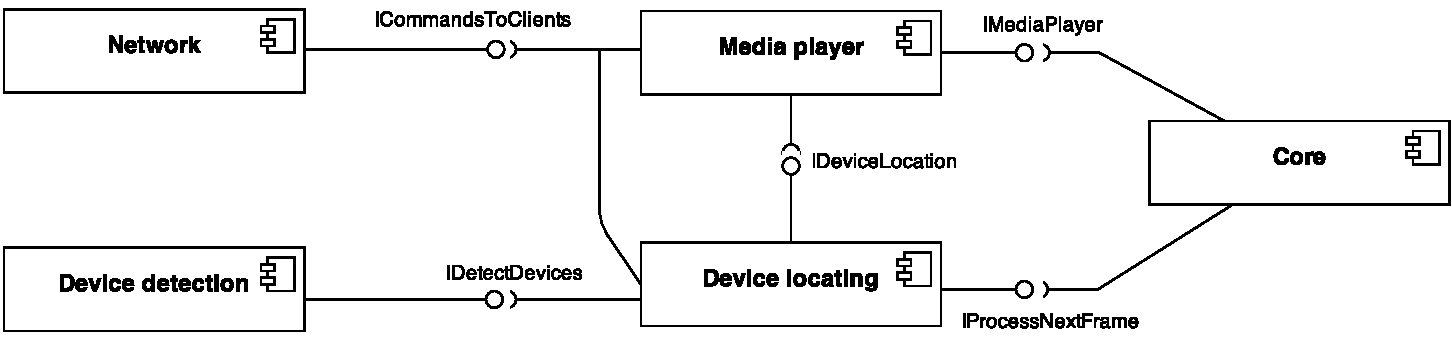
\includegraphics[width=16.2cm]{softwareArchitecture/component_diagram.pdf}
	\caption{Component diagram of server application}
	\label{fig:component_diagram_server}
\end{figure}


\paragraph{Network} is a component that provides interface which allows other components to communicate with clients. 
This includes broadcasting, unicasting and multicasting. 
It is also responsible for handling new connections from clients and creating new service.

\paragraph{Media player} is a component that provides simple interface consisting of start and stop command. 
It is responsible for playing actual media and timing for sending control commands to clients.

\paragraph{Device locating} is a component providing two interfaces. 
It must be able to handle incoming images and also it provides to other components locations of all connected clients.

\paragraph{Device detection} is a component that provides single interface. 
It accepts image as an input and it returns positions of possible devices.

\paragraph{Core} is a component that handles camera and manager's actions.


\section{Process view}
The process view shows concurrency and distribution of a system and system's processes.
It can also show communication between these units.
Process view can be described by activity diagrams.

You can see activity diagrams in Figures \ref{fig:activity_diagram_server} and \ref{fig:activity_diagram_client}. Note, that client application is sending signal action \emph{connect to server}, which is connected to server's event action \emph{new client connected}. 
 All clients connections are stored in datastore \emph{client list} and particular actions require all client connections to be able to send any information to clients.

\begin{figure}[h]
	\centering
		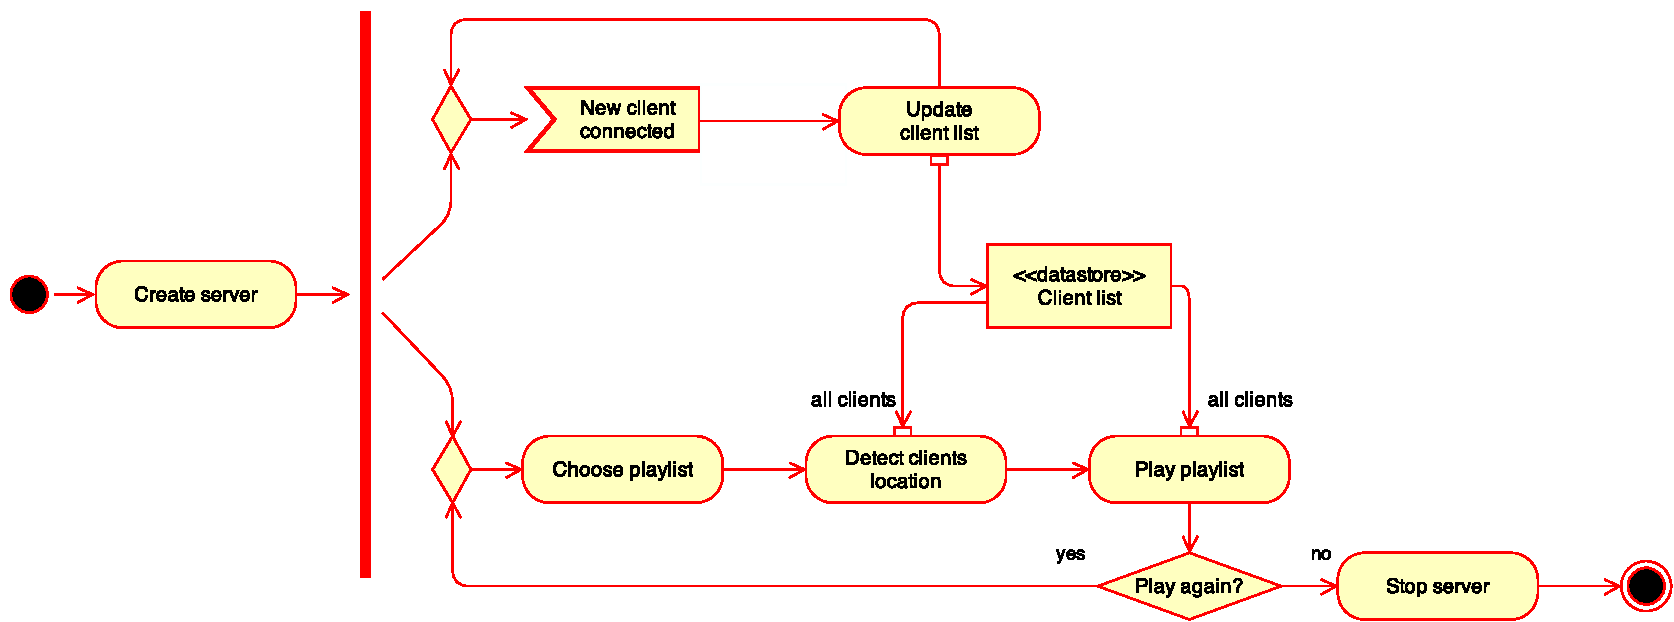
\includegraphics[width=16.2cm]{softwareArchitecture/activity_server.pdf}
	\caption{Activity diagram of server application}
	\label{fig:activity_diagram_server}
\end{figure}

\begin{figure}[h]
	\centering
		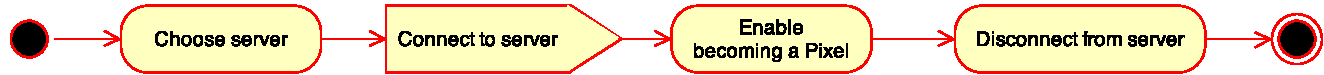
\includegraphics[width=16.2cm]{softwareArchitecture/activity_client.pdf}
	\caption{Activity diagram of client application}
	\label{fig:activity_diagram_client}
\end{figure}


\section{Physical view}
The physical view \cite{Kruchten:1995:VMA:624610.625529} describes a mapping of software onto hardware. 
It takes into account non-functional requirements of the system and it can be described by deployment diagrams.

Deployment diagram depicting physical view can be seen in Figure \ref{fig:architecture_deployment_diagram}.
According to requirement \refreq{N1}, there are two executable files deployed; one deployed to client device and second to server device.
There is also need for NTP\footnote{http://ntp.org/} server, which will maintain all connected devices synchronized.
To generalize the architecture design, the \emph{camera} device is treated as a separate device, which will only send its output to server device.

\begin{figure}[h]
	\centering
		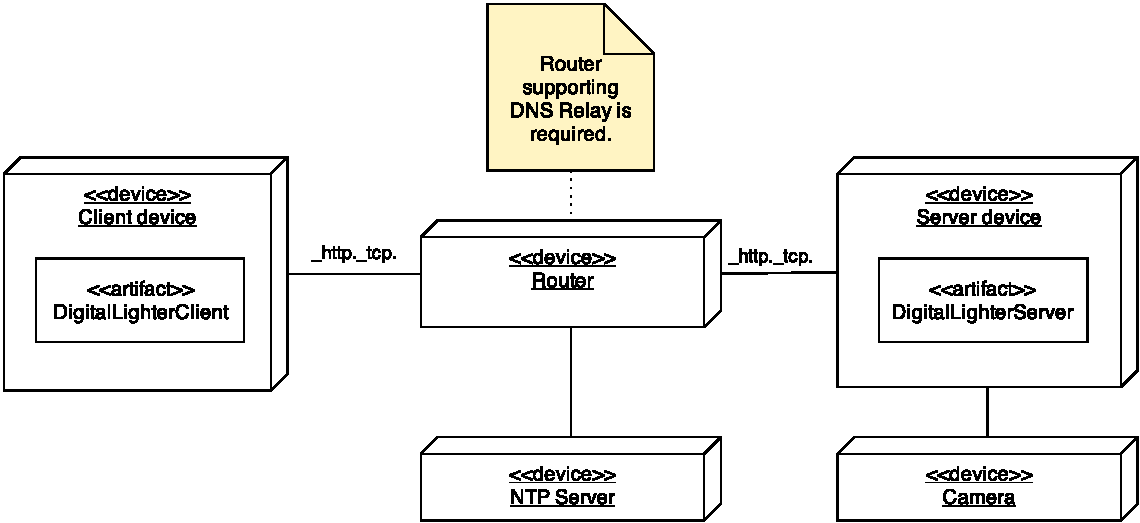
\includegraphics[width=15cm]{softwareArchitecture/deployment-diagram.pdf}
	\caption{Deployment diagram}
	\label{fig:architecture_deployment_diagram}
\end{figure}

\section{Scenarios}
Use case diagrams can be considered as scenarios, therefore introduced diagram \ref{img:usecase} in Requirements chapter can be considered as a scenario.

\section{Used design patterns}
\subsection{Strategy}
\subsection{Model-View-Controller}
\subsection{Observer}